\newpage

\hypertarget{abstract}{%
\section{Abstract}\label{abstract}}

Process models and Process Digital Twins frequently rely on
equation-oriented models to encode the behaviour of a factory. As
equation-oriented models grow in complexity, reasoning about their
structure becomes harder. This paper proposes an alternative workflow to
using degrees of freedom analysis to build equation-oriented models,
inspired by control systems. A set of properties for each unit operation
is chosen to fully specify the state; this is the set of properties you
design or control. These can then be replaced by other variables as
required for a specific case. This approach is demonstrated in the
equation-oriented modelling tool Pyomo. Benefits in model
interpretability, maintentance, initialisation, and application are
discussed. Various case studies demonstrate how processes can be
modelled in this manner, and how these techniques may prove advantageous
in a graphical user interface for process design. These methods may be
adopted by the process modelling community to make it easier to build
and maintain large equation-oriented models.

\newpage

\hypertarget{glossary}{%
\section{Glossary}\label{glossary}}

\textbf{AML}: Algebraic Modelling Language

\textbf{EOM}: Equation-Oriented Model

\hypertarget{introduction}{%
\section{Introduction}\label{introduction}}

Designing and operating chemical factories requires accurate,
comprehensive models of their behaviour. With the advent of more
computing resources and networked sites, process modelling has become
more critical than ever before. One way this is shown is in the rise in
popularity of Digital Twins, which try to make a complete and
comprehensive model of many different properties of entire sites and
their surroundings (Walmsley et al. 2024). As these models have become
larger, being able to understand all of the constraints within the
system simultaneously becomes harder and harder, making it harder to
run, interpret, or adjust the model.

A powerful tool to represent processes is equation-oriented algebraic
modelling, as processes often closely follow first-principles behaviour
and include non-linear dynamics, two things that equation-oriented
modelling excels at (Shacham et al. 1982). At its simplest,
equation-oriented modelling involves specifying equations to represent
the system, and solving those equations to find the unknown properties.
However, modern processes are very complex, and Digital Twin technology
means these models are built to be more integrated than ever before.
This results in very complex equation-oriented models (EOMs) and very
large sets of equations.

EOMs are usually specified in a declarative manner through Algebraic
Modelling Languages (AMLs). To help models remain understandable, newer
AMLs such as Pyomo apply software engineering principles of abstraction
and encapsulation so that the entire system does not always have to be
considered at once. This often means the person using the model does not
directly interact with the equations behind it, making it difficult to
know what is the best way to fully define the system and specify all
degrees of freedom. Combining multiple models, and adding additional
constraints further complicates the issue.

This article introduces a novel method to fully define an EOM. We
propose that the model developer should explicitly define an initial set
of variables to constrain. Then, those using the model can constrain
other variables, but only if they choose an another variable to
un-constrain. This method will simplify the process of squaring and
initialising a model. Our library, pyomo-replace, demonstrates some
advantages of this approach in the Pyomo and IDAES (Miller et al. 2018)
ecosystem, and the Ahuora Platform provides a case study of this
approach in a graphical application.

\hypertarget{literature-review}{%
\subsection{Literature Review}\label{literature-review}}

\hypertarget{equation-oriented-modelling}{%
\subsubsection{Equation-oriented
Modelling}\label{equation-oriented-modelling}}

Fundamentally, an EOM is simply a set of mathematical equations,
optionally with an objective function (Biegler 2010).

\[
\begin{aligned}
\min_{x} \quad & g(x) \\
\text{s.t.} \quad 
& \{c_i(x) = 0 : i = 1,...,m\} \\
& x \in X.
\end{aligned}
\]

The main parts of these equations are:

\begin{itemize}
\tightlist
\item
  \emph{Variables}:\(x\) represents a set of real numbers we do not know
  ahead of time, but solve the set of equations to find.
\item
  \emph{Constraints:} equality equations that are used to implicitly
  define the value, or solution space of, the variables. \(c_i\)
  represents a constraint expression that must equal zero for \(x\) to
  be considered a valid solution
\item
  \emph{Parameters}: a set of constants used in the constraints to
  calculate the variables.
\item
  An \emph{Objective Function} \(g(x)\): a function that is defined in
  terms of the variables, returns a value to minimise or maximise within
  the space of valid solutions. In square models, the goal is an exact
  solution so an objective function is not required, and we will
  disregard the objective function in most of this paper.
\end{itemize}

\hypertarget{equation-oriented-modelling-frameworks}{%
\subsubsection{Equation-oriented Modelling
Frameworks}\label{equation-oriented-modelling-frameworks}}

Variables, constraints, and objectives are fundamentally all that is
required in a mathematical model. However, over time additional
abstractions have been developed for easier programmatic creation and
manipulation of models, borrowing from conventional software development
data structures.

Traditionally, EOMs were built in special-purpose languages, such as
GAMS and AMPL. More recently they have moved to general-purpose
programming languages, which have extra tooling available that allow you
to build and initialise large EOMs programmatically (Jusevičius,
Oberdieck, and Paulavičius 2021). Some of the main modern
equation-oriented modelling tools include JuMP, built on Julia, and
Pyomo, built on python.

We will focus on Pyomo in particular here, as it was built with process
modelling in mind and has good libraries to aid in process modelling
(Hart, Watson, and Woodruff 2011). It is a framework for building
mathematical models that is written in Python . It includes tools to
manage abstraction and complexity in a mathematical model, and to define
initialisation routines and scaling factors to enhance numerical
stability. The equation-oriented modelling framework Pyomo includes the
following abstractions:

\begin{itemize}
\tightlist
\item
  Variables can be either \emph{Fixed} or \emph{Unfixed} respectively. A
  variable \(x_i\) that is fixed to a real value \(\bar{x}_i\) adds
  another equation \(f_i(x): x_i - \bar{x}_i\) to the set of constraint
  expressions, so that \(x_i = \bar{x}_i\). Because pyomo makes it easy
  to change which variables are fixed and which are unfixed, a model
  with the same structure can be used to solve for different variables.
\item
  Variables and constraints of similar form be grouped together through
  pyomo the pyomo \texttt{IndexedSet} functionality. A variable or
  constraint is added for each item in the set. Sets are constant - you
  can't add or remove items during solving - but they provide a
  generalisation that makes it easy to scale up, down, or modify
  problems for slightly different cases.\\
\item
  Variables can be grouped into \emph{Blocks}. Blocks can also have
  sub-blocks inside them, making a tree data structure\footnote{Variables
    and Blocks can be thought of like Files and Folders in a filesystem.
    Blocks only provide structure but no information, and can be nested
    inside each other, while variables contain the actual values in the
    model}.
\end{itemize}

Blocks are of particular interest here. Similar to how a class in
object-oriented programming provides encapsulation of more complex
functionality, Blocks are used to isolate the complex internal models of
different parts of a system. For example, in a mathematical model of a
factory, a block may be used to model each individual unit operation (a
pump, heater, tank, etc). The model inside the unit operation is
isolated from the higher level model, which only cares about the
properties of the fluid flowing in and out of the unit operation block.

Pyomo also includes some even higher level modelling extensions, which
are of particular relevance to Process Modelling:

\begin{itemize}
\tightlist
\item
  \emph{Pyomo.DAE} allows defining Differential Algebraic Equations
  across ``infinite'' sets that are discretised, automatically creating
  the necessary constraints to define derivatives and integrals
  (Nicholson et al. 2018). This is naturally useful in process modelling
  to create 1D simulations across time, taking in to account holdup,
  tank level, and so forth.
\item
  \emph{Pyomo.network} allows you to represent your model as a graph:
  Blocks become nodes in the graph, and they can be connected to other
  nodes via edges called ``arcs'' that define equality constraints
  between variables (Bynum et al. 2021). In many domains the graph view
  better represents the model structure. It also allows propagating
  initial values throughout a model. This is of particular importance as
  it allows sharing of information between distinct blocks. In a
  process, it is natural to use this interface to encode the connections
  between different unit operations, so that the output material of one
  unit operation is the input material to a successive unit operation.
\end{itemize}

Pyomo's construction techniques make it possible to create libraries of
pre-written blocks, containing all the constraints and variables to
model a piece of a physical system (Dowling and Biegler 2015). One such
library is IDAES-PSE. Built on top of Pyomo, it creates blocks to
represent chemical unit operations such as compressors, heaters, tanks,
and many more (Miller et al. 2018). It uses pyomo.DAE to represent time
as a continuous differentiable property, and Pyomo.network to represent
the connections between unit operations. Because the constraints are
abstracted, the user doesn't have to think too much about the
mathematical modelling - instead it is viewed a process simulation
platform.

\hypertarget{squaring-a-model}{%
\subsubsection{Squaring a model}\label{squaring-a-model}}

In order to solve a set of equations exactly, a ``square'' model is
required. This term is taken from linear algebra where a matrix must be
square to be invertible. In this context, it means that there must be
the same number of equations (constraints) as there are unknowns
(unfixed variables), for the problem to be well posed and have an exact
solution.

The difference between the two is described as the degrees of freedom. A
model that has more unknowns than constraints is said to have \(n\)
degrees of freedom, where \(n_{\text{degrees\ of\ freedom}}\) is given
by

\[
n_{\text{degrees\ of\ freedom}} =  n_{\text{variables}} - n_{\text{constraints}}
\]

Additionally, all the variables and equations must be linearly
independent. When building an EOM, the user will invariably come across
the problem of Degrees of Freedom; usually they will not have specified
the model sufficiently to be able to solve for an exact solution, i.e
\(n_{\text{degrees\ of\ freedom}} > 0\). Identifying how many and which
variables need to be ``fixed'' to make the model square can be a
challenge (Luyben 1996).

There are a number of techniques to make it easier to square a model.

One simple way is to include documentation about what typical fixed
variables are; this provides a starting point for a modeller that is
piecing together submodels developed by others. There are also automatic
methods to calculate the number of degrees of freedom via static
structural analysis, by subtracting the number of constraints from the
number of variables.

In (Bunus and Fritzson 2001), a method is proposed to help debug when a
model is singular, by using Dulmage-Mendelson Decomposition to identify
sets of constraints that are over-constrained or under-constrained.
These methods are commonly used in frameworks such as IDAES to help
ensure a square model is valid (Lee et al. 2024). However, while these
techniques are applicable to an entire ``flat'' system of equations, it
is hard to apply them to an individual subsection of a model without
understanding of what external constraints are applied. Some preliminary
work has been conducted to show that in some cases issues can be
identified in this level (Nilsson 2008), but it is limited in its
ability to detect errors and does not appear to have much uptake in
systems such as Pyomo. Additionally, Dulmage-Mendelson Decomposition
provides a big list of over-constrained or under-constrained components,
but does not provide any insight into which one of them should be
constrained.

Another technique is equation tearing, where a larger system is broken
up into a smaller system. This tries to decompose the system into a set
of equations that can be solved sequentially (Bahainv, Schichl, and
Neumaier 2016). This method is used by pyomo.network (Bynum et al. 2021)
as an initialisation strategy, but can also give some insight into what
is required to specify the model as each submodel can be considered
independently. However, this is less effective at identifying degrees of
freedom when the properties of the submodel are being set indirectly via
downstream properties.

Much of the research on squaring a model focuses on \emph{if} a model
has degrees of freedom or is fully specified, and \emph{where} the model
is over-specified. There is less research into \emph{why} the model is
over or under specified and \emph{what} a more sensible choice should
be. The problem of squaring a model has not often been analysed within
the domain that the models are used.

Taking a step back to look at the larger picture, Luyben et. al (Luyben
1996) observed and discussed the correlation between degrees of freedom
in design-time models and in control models, especially for reactors and
distillation columns. This is because the things you specify in design
time, such as inlet flow rates or outlet temperatures, need to be
controlled in the real factory, usually by valves. They argue that
calculating the number of controlled parameters in a plant is an easier
way to understand the degrees of freedom of a process than by trying to
analyse the number of equations and variables in a model that can be
adjusted independently.

Luyben et al.~raise an interesting link between design and control
specification that will be explored further in this paper. By embedding
the natural controllable properties in the model, and thinking about how
they are controlled in a similar way to how we design control systems,
we better bring the domain intuition into the problem of squaring a
model.

\hypertarget{method}{%
\section{Method}\label{method}}

In mathematical modelling, the modeller can choose what variables in a
model you want to specify, and which ones are calculated. The model has
complete freedom, so long as the final model is square with zero degrees
of freedom.

In the physical world, there are some things that can be adjusted, and
some that simply follow as a natural consequence. The closest thing to
``fixing'' a property, or holding a property constant, is control
theory. Let us consider a very simple model of a car's velocity:

\[
v = ky
\]

That is, the velocity \(v\) of a car on flat ground is equal to some
known performance constant \(k\) multiplied by the amount the
accelerator pedal is depressed, \(y\). If the accelerator is depressed
further, the final velocity of the car will increase. This can easily be
modelled in an AML, where fixing \(v\) or \(y\) results in a fully
defined system. In the physical world, the velocity of the car cannot be
set directly; rather, the manipulated variable must be the position of
the accelerator pedal. \(x\). From a control theory perspective, \(v\)
is the controlled variable, which has a fixed set point and effectively
replaces \(y\) in an EOM.

The intuition behind variable replacement is similar. There are some
variables that it is easy to think of as fully defining the system; we
will call them ``state variables''. They are all independent. All other
variables can be defined in terms of these state variables\footnote{This
  is analogous to the concept of a \emph{critical set} in combinatorial
  design theory.}. In this example, the position of the accelerator
pedal makes the most intuitive sense as the state variable, that is what
you set to control the car's speed.

It follows that if all state variables are fixed in a model, then the
model will have zero degrees of freedom. Fixing any other variable would
cause the system to be over-defined. Thus, similar to in control theory,
if one wanted to specify the car's velocity, you need to be able to
adjust the amount the accelerator pedal is depressed. This is the
fundamental principle behind variable replacement: start with all your
state variables defined, and then if you want to set something else, you
must choose a state variable to ``replace'', or ``unfix'' in Pyomo
language.

Starting with all the state variables fixed means you never have a
under-defined model. Unfixing a state variable every time you fix
something else means you never over-define your model. This makes it
much clearer how your model is intended to be used. Initialisation and
scaling methods also become much simpler if guesses are provided for all
the state variables, as you only need to define one way to
initialise/scale your model.

\hypertarget{formal-definition-of-variable-replacement-methodology}{%
\subsection{Formal Definition of Variable Replacement
Methodology}\label{formal-definition-of-variable-replacement-methodology}}

This section outlines how Variable Replacement is defined on an EOM,
borrowing terminology and concepts from the Pyomo equation-oriented
modelling ecosystem.

\hypertarget{mathematical-definition}{%
\subsubsection{Mathematical Definition}\label{mathematical-definition}}

An EOM be viewed mathematically as

\[
\mathcal{M} = (\hat{x}, C, F)
\]

where:

\(\hat{x} = (x_1,...,x_n )\) is a vector of \(n\) variables
\(\hat{x} ∈ ℝ^n\),

\(C = \{c_i: i = 1,...,m\}\) is a set of \(m\) functions such that
\(c_i(\hat{x}) = 0\) for all valid solutions of \(x\),

\(F = \{f_i: i ∈ S \}, S ⊆ \{1,...,n\}\) is an additional set of
functions of the form \(f_i(\hat{x}):= x_i - \bar{x}_i\), such that
\(f_i(\hat{x}) = 0\) for all valid solutions of \(x\), fixing the
variable \(x_i\) to the value \(\bar{x_i}\).

The set of feasible solutions can be given as:

\[
\mathcal{S} = \{C(\hat{x}) = 0, F(\hat{x}) = 0 \}.
\]

In other words, we need to find \(x\) such that
\(c(\hat{x}) = 0 \; ∀c ∈ C\) and \(f(\hat{x}) = 0 \; ∀f ∈ F\).

\hypertarget{degrees-of-freedom}{%
\subsubsection{Degrees of freedom}\label{degrees-of-freedom}}

The number of degrees of freedom of the model is defined as:

\[
\text{DoF} = |\hat{x}| - |F| - |C| 
\]

Or the number of variables minus the number of fixed variables minus the
number of constraints.

If all constraints are independent, when DoF is zero there is an exact
solution. If there are more constraints, the model is over-defined and
degrees of freedom is negative. If there are more variables, then there
are a range of possible solutions.

\hypertarget{replacement}{%
\subsubsection{Replacement}\label{replacement}}

Variable replacement is a method of changing which variables in the
model are fixed. We start with a fully defined model
\(\mathcal{M} = (\hat{x}, C, F)\) such that:

\[
DoF(\mathcal{M}) = |\hat{x}| - |F| - |C|  = 0
\]

Fixing a variable \(V_i\) at index \(i\) involves adding a constraint
\(f_i\) to \(F\). We define \(F' = F ∪ \{f_i\}\). However, if this is
used in a model, \(DoF((\hat{x},C,F')) = -1\) so the model would be
over-defined and potentially have no solutions.

To solve this, we also choose an existing fixed variable to unfix, by
removing it's constraint \(f_j\) from \(F\). This gives us a new set of
constraints

\[
F_{new} = (C \backslash \{f_j\}) ∪ \{f_i\}
\]

and a new model

\[
\mathcal{M}_{new} = (\hat{x},C,F_{new})
\]

that maintains the condition that \(DoF(\mathcal{M}_{new}) = 0\).

\hypertarget{an-example}{%
\subsubsection{An example}\label{an-example}}

Returning to the model of a car acceleration:

\[
v = ky
\]

We can define a vector of variables \(x\):

\[
\hat{x} :=
\begin{pmatrix}
v \\
k \\
y \\
\end{pmatrix}
\]

And the equations can be rearranged into a functional form where C(x) =
0:

\[
C :=
\begin{Bmatrix}
x → ky - v\\
\end{Bmatrix}
\]

As \(|\hat{x}| - |C| = 2\), we need to fix two variables to have zero
degrees of freedom. These two variables will become our state variables,
the ones ``fixed by default'' in the model.

Choosing which variables are the state variables is an important step in
the Variable Replacement Methodology. It is best to choose variables
that are decision variables (either variables chosen during design, or
manipulated via the control system) rather than output or dependent
variables.

In this case, \(k\) is a design variable, as it is chosen based on how
the car is manufactured. \(y\) is a operational variable that can be
directly manipulated at any stage. \(v\) is a dependent variable that is
controlled via the other two. As \(k\) and \(y\) are both decision
variables, it is appropriate they are used as the state variables.

If we specify \(k = 1, y = 0.2\), then we can define \(F\) as follows:

\[
F :=
\begin{Bmatrix}
\hat{x} → k - 1 \\
\hat{x} → y - 0.2  \\
\end{Bmatrix}
\]

This defines the initial model, which can be solved to an exact
solution. If the modeller wants to design to a specific velocity
\(v = 7.5\), they cannot fix this variable unless they choose something
else to unfix. They must unfix one of the state variables, either \(k\)
or \(y\). For a control case, \(y\) may be replaced. Using the variable
replacement approach, this would define an update set of fixed
variables:

\[
F' :=
\begin{Bmatrix}
\hat{x} → k - 1 \\
\hat{x} → v - 7.5  \\
\end{Bmatrix}
\]

\hypertarget{a-reference-implementation-pyomo-replace}{%
\subsection{A reference implementation:
pyomo-replace}\label{a-reference-implementation-pyomo-replace}}

To aid in evaluating the advantages of a variable replacement approach
to equation-oriented modelling, we have created a small python package
built on IDAES and pyomo, called pyomo-replace. It demonstrates the
principles of variable replacement in a format as similar as possible to
standard IDAES modelling, to make it easier to draw comparisons between
the two approaches.

Pyomo-replace contains methods to keep track of the state variables in
an IDAES model, and what variables are replacing them. The list of state
variables and replacements can be easily printed to the screen to help
explain the model structure.

A full explanation of the pyomo-replace library, including a link to the
source code, is included in the appendix.

\hypertarget{properties-of-a-variable-replacement-approach-to-equation-oriented-modelling}{%
\section{Properties of a Variable Replacement approach to
Equation-oriented
Modelling}\label{properties-of-a-variable-replacement-approach-to-equation-oriented-modelling}}

This method of replacing state variables to define a model does not
fundamentally change the model itself. However, specifying a model in
this way provides some guarantees and useful properties that traditional
equation-oriented methods lack.

A useful analogy may be in the study of programming language theory.
Functional and Imperative programming languages are both turing
complete, but certain problems are better represented in an imperative
language, while other problems are more simply expressed in a functional
manner. Likewise, static typing systems do not change the correctness of
a program, but they do make it simpler to validate and reason about the
program.

Variable replacement enforces a degree of regularity in the blocks that
make up models, and in the overall structure. It provides a different
paradigm in which to reason about equation-oriented systems.

\begin{enumerate}
\def\labelenumi{\arabic{enumi}.}
\tightlist
\item
  It fundamentally removes the problem of Degrees of Freedom when
  defining a model.
\item
  Switching between different types of analysis for design versus
  operation becomes easier.
\item
  It standardises initialisation routines, as long as guesses are
  provided for state variables.
\item
  The coupling of variables adds a level of interpretability to the
  model, which makes it easier to maintain and manipulate models.
\end{enumerate}

\hypertarget{removing-the-problem-of-squaring-a-model}{%
\subsection{Removing the problem of Squaring a
Model}\label{removing-the-problem-of-squaring-a-model}}

To have a square model, you must have the same number of unknowns, or
unfixed variables, as equations, i.e
\(n_{\text{degrees\ of\ freedom}} = 0\).

Traditional model libraries such as IDAES provide the equations, and
then all that is required is to specify enough variables that the number
of variables equals the number of unknowns. This can be done by
repeatedly fixing variables in a part of a model that is not already
over-defined\footnote{i.e You must fix variables that are part of a
  Dulmage-Mendelson under-constrained set.}, until the model is fully
defined. Incorrect degrees of freedom has been identified as a common
source of errors in EOMs, and checking the degrees of freedom is the
first recommended step to diagnose problems (Lee et al. 2024). Newer
analysis methods, such as Dulmage-Mendelson Decomposition do make this
simpler, but it is still an iterative process.

Using a Variable Replacement approach, a set of state variables would be
already defined by the model library, so the user would not need to
square the model. There are zero degrees of freedom \emph{by
definition}. If a problem requires a variable to be fixed that is not a
state variable, an appropriate\footnote{i.e A state variable that would
  be part of the Dulmage-Mendelson over-constrained set if the other
  variable was fixed and nothing was unfixed} state variable must be
unfixed too. As we add a degree of freedom every time we remove a degree
of freedom, they `cancel out' guaranteeing that we will continue to have
a square model. This eliminates an entire class of errors with practical
application of EOMs.

\hypertarget{switching-between-different-types-of-analysis}{%
\subsection{Switching between different types of
analysis}\label{switching-between-different-types-of-analysis}}

We have previously discussed using the car example that some state
variables are design state variables (i.e \(k\)), and some are
manipulated variables (i.e \(y\)), and all other variables are dependent
(i.e \(v\)).

A design problem would involve finding an appropriate for the design
state variables, by calculating a desired \(k\). In an operation case,
\(k\) is fixed and known, but an appropriate value of \(y\) may be
required. To turn a design case into an operation case, all that is
required is to fix all the design variables, which can be done un-doing
any replacements that have happened on them. With the additional
metadata on what variables are replacing what, it becomes much easier to
create tools to switch between design and operation modes.

Likewise, a robustness test typically involves fixing only the decision
variables (both design and operation) and calculating how sensitive the
dependent variables are to changes. Again, this is easy to do in the
variable replacement framework by simply undoing all replacements, as
the decision variables are the state variables.

\hypertarget{simplified-initialisation}{%
\subsection{\texorpdfstring{Simplified Initialisation
}{Simplified Initialisation }}\label{simplified-initialisation}}

Initial guesses greatly increase the robustness of solving EOMs.
Modelling toolboxes such as IDAES provide methods to automatically
define initial guesses based on fixed variables. However, if different
variables are fixed to the ones the modelling library expects, these
methods will not provide any benefit, and may even cause additional
problems.

\begin{figure}
\centering
\includegraphics{assets/initialisation-methods.drawio.png}
\caption{Alternative initialisation routine, making use of state
variables to avoid the need for different initialisation methods.}
\end{figure}

The concept of ``State Variables'' can simplify this process, by
splitting the initialisation into two parts. First, the initialisation
methods can calculate initial values of all variables based on the
values or guesses of the state variables. Then, once the model has been
initialised in a sensible location, any state variables that are
replaced (i.e, were guesses) can be unfixed, and the variables that are
replacing them can be fixed back to their original values. The block can
then be re-solved to calculate the correct value of any ``guessed''
state variable.

This limits the logic in initialisation routines, as only one
initialisation method is required be required. It does require that
initial guesses are provided for all the state variables, but this is a
reasonable tradeoff. This standardises the initialisation process to
work across all sets of fixed variables, while still giving the model
library developer freedom to develop whatever initialisation method they
think is best.

A test with the IDAES turbine model demonstrates this to be the case. A
turbine model was constructed, with 100 mol/s of 200°C steam at 1MPa, an
isentropic efficiency of 50\% and a pressure drop of 900 kPa. Different
combinations of variables were fixed, and then the model was initialised
and then solved with those fixed variables using IDAES's standard
initialisation routines. Idaes's initialisation routines check which
variables are fixed and perform different initialisation methods
accordingly.

This was compared to the same model, at the same conditions, but with
initialisation performed first using a guess for efficiency and work.
Subsequently, efficiency and work are unfixed and the model is solved
using the specified variables.

\begin{longtable}[]{@{}lll@{}}
\caption{Comparison of solving success with different combinations of
variables, with and without staged initialisation.}\tabularnewline
\toprule
\begin{minipage}[b]{0.19\columnwidth}\raggedright
Fixed Variables\strut
\end{minipage} & \begin{minipage}[b]{0.36\columnwidth}\raggedright
Standard IDAES Initialisation\strut
\end{minipage} & \begin{minipage}[b]{0.37\columnwidth}\raggedright
Staged Initialisation Approach\strut
\end{minipage}\tabularnewline
\midrule
\endfirsthead
\toprule
\begin{minipage}[b]{0.19\columnwidth}\raggedright
Fixed Variables\strut
\end{minipage} & \begin{minipage}[b]{0.36\columnwidth}\raggedright
Standard IDAES Initialisation\strut
\end{minipage} & \begin{minipage}[b]{0.37\columnwidth}\raggedright
Staged Initialisation Approach\strut
\end{minipage}\tabularnewline
\midrule
\endhead
\begin{minipage}[t]{0.19\columnwidth}\raggedright
Mechanical Work \& Efficiency\strut
\end{minipage} & \begin{minipage}[t]{0.36\columnwidth}\raggedright
Success\strut
\end{minipage} & \begin{minipage}[t]{0.37\columnwidth}\raggedright
Success\strut
\end{minipage}\tabularnewline
\begin{minipage}[t]{0.19\columnwidth}\raggedright
Work \& Outlet Pressure\strut
\end{minipage} & \begin{minipage}[t]{0.36\columnwidth}\raggedright
Initialisation Error\strut
\end{minipage} & \begin{minipage}[t]{0.37\columnwidth}\raggedright
Success\strut
\end{minipage}\tabularnewline
\begin{minipage}[t]{0.19\columnwidth}\raggedright
Efficiency \& Outlet Pressure\strut
\end{minipage} & \begin{minipage}[t]{0.36\columnwidth}\raggedright
Success\strut
\end{minipage} & \begin{minipage}[t]{0.37\columnwidth}\raggedright
Success\strut
\end{minipage}\tabularnewline
\begin{minipage}[t]{0.19\columnwidth}\raggedright
Work \& Pressure Ratio\strut
\end{minipage} & \begin{minipage}[t]{0.36\columnwidth}\raggedright
Initialisation Error\strut
\end{minipage} & \begin{minipage}[t]{0.37\columnwidth}\raggedright
Success\strut
\end{minipage}\tabularnewline
\begin{minipage}[t]{0.19\columnwidth}\raggedright
Efficiency \& Pressure Ratio\strut
\end{minipage} & \begin{minipage}[t]{0.36\columnwidth}\raggedright
Success\strut
\end{minipage} & \begin{minipage}[t]{0.37\columnwidth}\raggedright
Success\strut
\end{minipage}\tabularnewline
\bottomrule
\end{longtable}

\hypertarget{interpretability-and-model-maintenance.}{%
\subsection{Interpretability and model
maintenance.}\label{interpretability-and-model-maintenance.}}

In conventional programming languages, type systems are frequently used
to increase a programs interpretability. In many cases, typing is not
strictly necessary for a program to run, but it bakes in crucial context
about what the expected inputs and outputs of a piece of code are. While
this is generally more verbose than the equivalent untyped code, many
developers find this invaluable in helping to understand the system.

The replacement system works in a similar manner, as it bakes in more
context to the model. Similar to a type system in a programming
language, this increases the model's interpretability and
maintainability. Technically, it doesn't matter which state variable a
model is replacing; just which variables are fixed and which are
unfixed. However, having that context makes understanding \emph{why} a
variable needs to be fixed much clearer.

Admittedly, interpretability is a subjective concept. Thus it will be
illustrated through a series of examples differing in scale and
complexity, and reasoning will be provided as to why the extra context
that Variable Replacement provides benefits that case.

\hypertarget{example-1-a-single-compressor}{%
\subsubsection{Example 1: A single
Compressor}\label{example-1-a-single-compressor}}

A simple compressor model, using a traditional modelling toolbox, may
include the following variables as shown in Figure \ref{compressor-dof}.

\begin{figure}
\centering
\includegraphics{assets/compressor-5dof.drawio.png}
\caption{Variables in a simple compressor model. \label{compressor-dof}}
\end{figure}

The equivalent model, using a variable replacement approach, would have
state variables already defined by the developer of the Compressor Unit
Model (Figure \ref{compressor-sv-defined}).

\begin{figure}
\centering
\includegraphics{assets/compressor-sv.drawio.png}
\caption{Variables in a simple compressor model, with everything that is
not a fixed greyed out. \label{compressor-sv-defined}}
\end{figure}

This is more interpretable, as it provides extra context: it explains
what the model developer expected was most likely to be fixed.

However, depending on the problem, different variables may be fixed. For
example, the outlet pressure may be known instead of the mechanical
work. In a traditional system, you would just fix the outlet pressure
instead of the mechanical work (Figure
\ref{compressor-fixed-traditional}).

\begin{figure}
\centering
\includegraphics{assets/compressor-fixed-outlet.drawio.png}
\caption{Fully specified compressor model using a traditional approach.
\label{compressor-fixed-traditional}}
\end{figure}

The equivalent model, using a variable replacement approach, would
require explicitly replacing the mechanical work state variable. This
would create a link between the two variables to show what Mechanical
work was replaced by (Figure \ref{compressor-replacement}).

\begin{figure}
\centering
\includegraphics{assets/compressor-replaced.drawio.png}
\caption{Compressor model using the variable replacement system, with
Outlet Pressure replacing Mechanical Work.
\label{compressor-replacement}}
\end{figure}

This provides a natural form of documentation for the model: The outlet
pressure is being specified because it is needed to calculate the
mechanical work of the compressor. On large systems, this explanation
becomes particularly beneficial, as it becomes harder to identify why a
property needs to be set, particularly when degrees of freedom are being
specified indirectly.

\hypertarget{example-2-modifying-a-flowsheet}{%
\subsubsection{Example 2: Modifying a
flowsheet}\label{example-2-modifying-a-flowsheet}}

EOMs are generally considered as a finished product, and their evolution
and development is ignored. However, in practice EOMs are built like
pieces of software; iteratively and incrementally over time\footnote{A
  good explanation of iterative vs incremental development is discussed
  by Jeff Patton at
  \url{https://jpattonassociates.com/dont_know_what_i_want/}}. A model
is generally built by applying a series of modifications to a simple
model, including:

\begin{itemize}
\tightlist
\item
  Changing which variables are fixed (In variable replacement, this
  would be replacing variables, in a Degrees of freedom approach, this
  would be fixing and unfixing variables)
\item
  Adding a new variable with a corresponding constraint to define it
  (e.g defining a custom calculated property)
\item
  Adding a new set of variables and corresponding constraints (e.g
  adding an additional unit operation to a model)
\item
  Replacing a constraint or set of constraints with an alternative
  specification (e.g switching to a different formulation of a compound
  or unit operation's characteristics)
\item
  Removing a set of variables and/or constraints from a model (e.g
  removing a unit operation that is not required in a model)
\item
  Replacing a fixed variable with a constraint to define that variable.
\end{itemize}

Because the number of unfixed variables must always be the same as the
number of constraints, when unfixed variables are added or removed, the
same number of constraints need to be added or removed too. However,
this is a non-trivial process. If a variable is removed, which
constraint should be removed with it? This problem compounds when you
are removing multiple variables and constraints simultaneously.

\begin{figure}
\centering
\includegraphics{assets/deleting-replacement.drawio.png}
\caption{Deleting the pump from a flowsheet is handled elegantly as the
fixed variables are coupled to specific state variables.}
\end{figure}

Consider this model of a pump connected to a heater, with all the state
variables defined. The inlet conditions are state variables, and so is
the mechanical work of the pump, and the heat duty of the heater.
However, the mechanical work and heat duty are replaced by the
temperature and pressure of the outlet; i.e the temperature and pressure
will be used to calculate mechanical work and heat duty.

When the pump is removed from the flowsheet, the intermediate stream
becomes the new inlet, and thus its temperature, pressure, and flow will
need to be fixed. Because the outlet pressure was replacing Mechanical
Work on the pump, and the pump has been removed, outlet pressure no
longer needs to be fixed. Thus, the model is still fully specified.

\begin{figure}
\centering
\includegraphics{assets/deleting-traditional.drawio.png}
\caption{Using a traditional modelling methodology, there is no coupling
of variables, so when the pump is deleted there is no intuition what
variables to remove.}
\end{figure}

Using a traditional modelling methodology, there is no coupling of
variables, so when the pump is deleted there is no information provided
on what variables to remove. There are two options:

\begin{enumerate}
\def\labelenumi{\arabic{enumi}.}
\tightlist
\item
  Fix the inlet conditions automatically, similar to the strategy in
  variable replacement. This will leave you with an over-defined model,
  as pressure would still be fixed on the outlet also. The modeller
  would have to manually unfix outlet pressure to again have a solvable
  model.
\item
  Don't fix the inlet conditions automatically. This would leave you
  with an under-defined model, and the modeller would have to choose two
  variables to fix (e.g inlet temperature and flow) to again have a
  solvable model.
\end{enumerate}

Both of these options require manual intervention from the modeller, as
there is no clear path to maintain a solvable model. In comparison, when
fixed variables are coupled to a set of state variables, it is easy to
see when to unfix the variable: when the state var it is connected to is
removed.

\hypertarget{analysing-interpretability}{%
\subsubsection{Analysing
interpretability}\label{analysing-interpretability}}

Whether the method of replacement improves interpretability and
maintainability is a subjective question. Nonetheless, these examples
demonstrate the basic properties of Variable Replacement, and the
advantages that it can provide in understanding the relationships
between fixed variables in the system, without needing to dig into the
underlying mathematical formulations. This also makes it simpler to
modify a model and maintain a solvable state. However, similar to typed
languages in software development, the realisable benefit may depend on
the use case.

\hypertarget{case-studies}{%
\section{Case Studies}\label{case-studies}}

To help demonstrate the potential of a Variable Replacement approach to
designing systems built on EOMs, this section includes three examples.
The first discusses a geothermal plant, showing how Variable Replacement
makes it easier to keep track of the sources of variability in the
system. The second discusses a Dynamic Tank, showing how Variable
Replacement can work with a time-based problem. The third discusses how
variable replacement makes it easier to create User Interfaces (UIs) for
building equation oriented models from sets of pre-configured equations.

\hypertarget{geothermal-power-plant}{%
\subsection{Geothermal Power Plant}\label{geothermal-power-plant}}

\begin{figure}
\centering
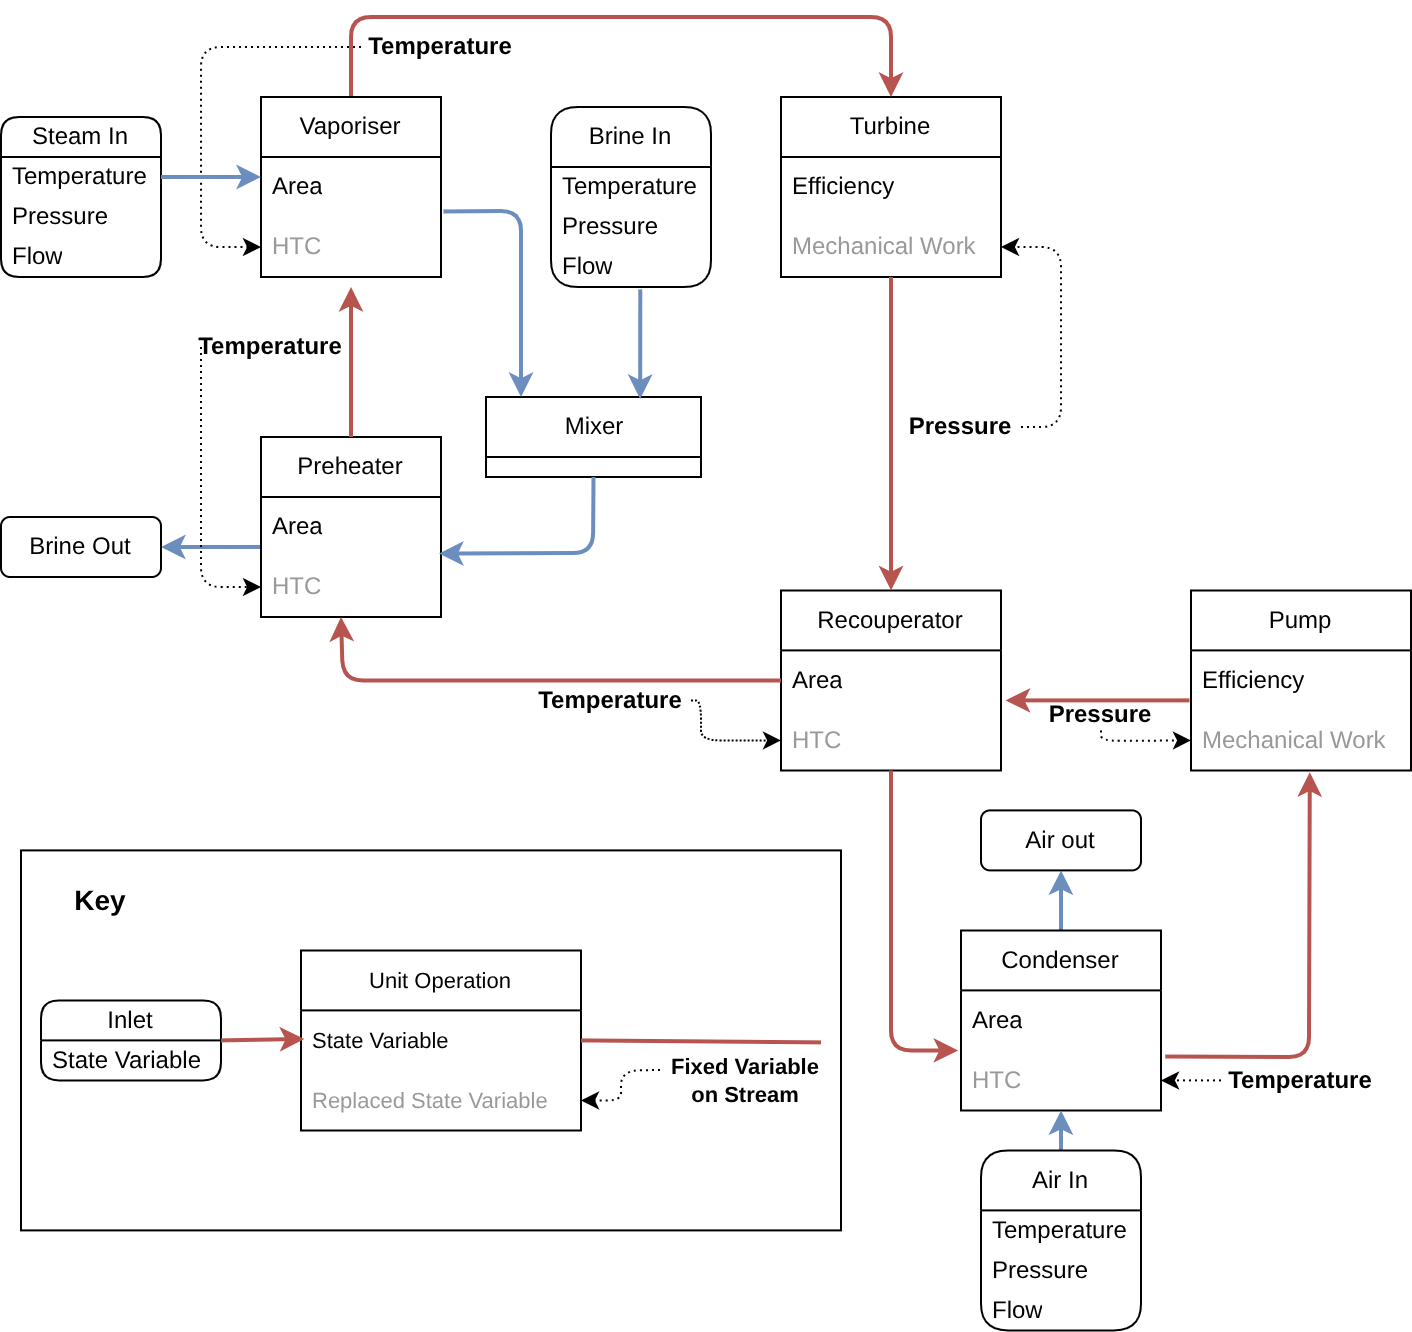
\includegraphics{assets/geothermal-replacement.drawio.png}
\caption{Flow Diagram of a fully specified Geothermal Power Plant,
demonstrating which state variables are being replaced.}
\end{figure}

A model of a geothermal plant, outlined in (Severinsen et al. 2024) is
shown here as a test case. This model includes four heat exchangers (the
condenser, recouperator, preheater, and vaporiser), one turbine, and one
pump. Each of these unit operations contribute one or two degrees of
freedom: The heat exchangers need Area and Heat Transfer Coefficient
(abbreviated as HTC) to be specified, and the Turbine and Pump both need
efficiency and mechanical work. Additionally, the Steam Inlet, Air
inlet, and Brine inlet need their temperature, pressure, and flow to be
specified, as they are not connected to any upstream unit operations.

However, the plant data includes stream pressures and temperatures, so
the mechanical work and heat transfer coefficients are not actually set
in this model. Instead, they are replaced with the pressure or
temperature measured on the stream flowing out of the unit operations.
Because of the replacement system, it is easy to see exactly why each of
these temperatures and pressures need to be specified, and why the other
streams (e.g from the recouperator to the condenser) do not need their
properties specified.

Those familiar with control systems may note that the variable
replacement approach for the pump looks similar to the control scheme of
a pump in a P\&ID Diagram, where the amount of work the pump does is
controlled by a PID tuner that reads from a pressure sensor. The concept
is not exactly analogous for heat exchangers, where the sizing is
pre-determined, but the parallels may be helpful in gaining an intuition
for how degrees of freedom replacement behaves.

Of particular note is the flow in the brine inlet. The factory does not
record the brine flow in, however it does record the total flow out.
Thus, we can replace the Brine inlet flow with the Total flow, and the
Brine flow will be back-calculated. Note that the brine outlet flow is
specified much later downstream from the brine inlet. When this happens
in conventional Degree of Freedom replacement systems, it can be very
hard to understand why the brine outlet flow needs to be specified. By
using a Variable Replacement approach, it is immediately obvious.
Specifying stream properties downstream of an operation, sometimes
significantly downstream, is a common practice when modelling, and
Variable replacement makes it easier to understand why these properties
need to be specified.

\hypertarget{dynamic-tank}{%
\subsection{Dynamic Tank}\label{dynamic-tank}}

\begin{figure}
\centering
\includegraphics{assets/dynamics.drawio.png}
\caption{A model of a tank with valves controlling the inlet and the
outlet. Properties with an asterisk (*) next to them are not
time-indexed. The tank outlet pressure is referenced by the PID
controller, but is not a state variable.}
\end{figure}

A dynamic flowsheet allows us to test a different aspect of our system:
how indexed variables are handled. In this flowsheet, we have a steam
tank, modelled as a Heater in idaes, with a constant volume and an inlet
and outlet valve controlling the flow rate in and out of the tank. The
flow into the tank is controlled by a PID controller, which is targeting
a certain outlet pressure within the tank.

Both the valves have two state variables: the valve coefficient, and the
valve opening fraction. However, the valve coefficient is a constant
property; it cannot be changed throughout the simulation. To indicate
this, we have included an asterisk (*) next to them. In contrast, the
valve opening fraction can be changed over time, and so in IDAES it is
indexed by time. It is actually a set of variables, one variable for
every time step across the simulation. Variables with an asterisk next
to them cannot replace variables without an asterisk and vice versa,
because the time indexed variables actually represent many degrees of
freedom, while the others only represent one degree of freedom. However,
in almost all cases it makes sense to treat the variable across time in
the same manner (either you want to fix it, or you don't.)

In this flowsheet, only two replacements are required. The first
involves replacing the inlet flow with the outlet pressure. These can be
replaced because a pressure difference between the inlet and the outlet
is what drives the fluid through the system. The flow can be calculated
from the valve pressure-flow correlation. Both pressure and flow are
time-indexed properties, so they each represent the same number of
degrees of freedom. Note that with our initialisation strategy, we start
with a guess for flow, and then we initialise with that. After
initialisation is completed, the flowsheet re-solves with the correct
outlet pressure fixed, recalculating what the true flow value is.

The second replacement involves replacing the valve opening fraction
with the setpoint. The PID controller sets the value of the valve
opening fraction, so the valve opening fraction no longer needs to be
specified. This goes against the general logic of variable replacement.
However, the setpoint of the PID controller needs to be specified. So we
can add a replacement to say that the setpoint replaces the valve
opening fraction. This is a simple solution that can be done when the
PID controller is connected up to the valve opening fraction.

Initial Material Accumulation and Initial Energy Accumulation can be
treated as additional state variables if it is appropriate. It would be
feasible to use the replacement logic to replace them with Initial
Material Holdup and Initial Energy Holdup. However, typically dynamic
flowsheets start with a steady-state assumption, and all accumulation
terms are fixed to zero.

This case study successfully demonstrates that the variable replacement
logic can easily be extended to more complex flowsheet scenarios
involving dynamics or other indexed variables.

\hypertarget{ahuora-digital-twin-platform}{%
\subsection{Ahuora Digital Twin
Platform}\label{ahuora-digital-twin-platform}}

\begin{figure}
\centering
\includegraphics{assets/ahuora-interface.png}
\caption{A Heat pump in the Ahuora Platform.}
\end{figure}

While this paper has focused on the theoretical advantages of a Variable
Replacement methodology, a major reason we have developed this method of
variable replacement is because it works particularly well in a
graphical user interface.

The Ahuora Digital Twin Platform is a web-based process simulation
environment. It is built using IDAES and Pyomo as the equation-oriented
modelling libraries as the simulation backend.

Each unit operation has a set of state variables, where the user can
enter a value, and a set of calculated variables, which cannot be
entered by the user. If a user wants to fix a calculated variable, an
appropriate state variable has to be chosen and ``replaced''. This makes
the state variable a ``guess'': the user still needs to enter a value,
but it is shown with no background color, to indicate to the user that
it will be calculated when the flowsheet is solved. A message tells the
user what variable is replacing it. The calculated variable then shows
up like a state variable, with a message to show which variable it is
replacing. This ensures the user is informed about which variable is
being replaced by which.

\begin{figure}
\centering
\includegraphics{assets/ahuora-replacement.png}
\caption{Variable replacement on a Compressor model in the Ahuora
Platform.}
\end{figure}

In the example image, the ``Pressure Drop'' state variable is fixed at 0
kPa. The ``Mechanical Work'' state variable in the Compressor is being
replaced by the Pressure at the outlet stream. An initial guess for
``Mechanical Work'' may still be entered, which is updated to the
correct value, which is based on the pressure specified at the outlet,
when the model solves.

Before using the variable replacement approach, we only limited the user
to a fixed set of choices of variables for each unit operation. However,
this reduced functionality significantly as there was no method to
specify unit models indirectly, such as through downstream properties.
We thought about trying a degrees of freedom approach, but were
concerned that it would be much too confusing as it didn't provide the
user with any direction on how to get started.

One of the major advantages of Variable Replacement that we have noticed
in a GUI is that it provides additional context for unit operations. In
a GUI program, it is very easily to visually show that context by
styling fixed State Variables, guesses, and calculated variables
differently, and to show the links between variables.

Working with a GUI also means that adding and removing unit operations
is common, and Variable Replacement provides a sensible way to deal with
adding or removing unit operations. When a unit operation is added, it's
state variables and inlet ports are fixed by default to ensure the
degrees of freedom are still zero. When a unit operation is removed,
anything that is replacing it's state variables is also unfixed, and any
inlet ports that were previously connected to the outlet of the unit
operation are fixed, again keeping the degrees of freedom at zero.

The GUI also does not provide any way to write custom initialisation
routines, because these are usually specified as python code and can be
quite complex, so it is out of scope of the project. However, the
multi-stage initialisation that naturally works with variable
replacement helps to improve the reliability of solving. As guesses are
specified for the state variables, these can be used in the
initialisation routine. In particular, this enables us to specify any
set of variables to define the conditions of an inlet stream, whereas
IDAES does not have initialisation routines for any set of state
variables and is typically limited to only a certain set of properties.

\hypertarget{conclusion}{%
\section{Conclusion}\label{conclusion}}

Variable replacement provides an alternative way of maintaining a square
model in an equation-oriented framework, particularly when scaling up to
larger EOMs.

If state variables are defined on each block added to a model, those who
use the model do not need to first square the problem. Degrees of
freedom are kept at zero through any changes that are made to the
flowsheet. The coupling between state variables and fixed variables
provides a more interpretable way of reasoning about the model, bringing
the relationships between variables to the forefront. Additionally, a
set of state variables and initial guesses for them makes it simpler to
build initialisation and scaling methods. The Ahuora Digital Twin
Platform provides a case study on how this is beneficial, particularly
when using a GUI tool for modelling.

While this paper introduces Variable Replacement as a method and purview
it's potential benefits, further research is required to systematically
evaluate the interpretability and initialisation advantages across
different types of EOMs. Nonetheless, these techniques hold promise to
standardise the creation and use of libraries of EOMs. This would enable
equation-oriented modelling to be used in a more maintainable way on
large projects, such as Process Digital Twins, in the future.

\newpage

\hypertarget{appendix}{%
\section{Appendix}\label{appendix}}

\hypertarget{pyomo-replace-source-code}{%
\subsection{Pyomo-Replace Source code}\label{pyomo-replace-source-code}}

A sample implementation of replacement logic in Pyomo, along with the
initialisation tests and geothermal model example, are available at
\url{https://github.com/bertkdowns/pyomo-replace}.

\hypertarget{introduction-to-pyomo-replace}{%
\subsection{Introduction to
Pyomo-replace}\label{introduction-to-pyomo-replace}}

Pyomo-replace is a simple library to keep track of the state variables
in an IDAES model, and what variables are replacing them. The list of
state variables and replacements can be easily printed to the screen to
help explain the model structure.

In Pyomo, an EOM is specified as a set of Blocks, with each block
containing variables and constraints between variables. A Block may
contain Ports, which provide a method of connecting Blocks together.

A Port is simply a collection of variables on a block. A port is
specified to be either an Inlet Port or an Outlet Port. An Inlet port
may be connected to an Outlet port containing an equivalent collection
of variables. The inlet and outlet port do not need to be on the same
block. Connecting two ports creates an equality constraint between the
variable on the Outlet and the variable on the Inlet, that is, the
variable on the inlet is defined to be equal to the corresponding
variable on the outlet port.

The IDAES framework makes it easy to model chemical engineering problems
in pyomo. An equation-oriented model typically represents a chemical
flowsheet, a Block typically represents a unit operation, and Inlet and
Outlet Ports represent inlets and outlets of a unit operation.
Pyomo-replace is specifically targeted to representing these types of
EOMs.

\hypertarget{state-variables}{%
\subsubsection{State Variables}\label{state-variables}}

Because each block contains a set of variables and constraints, it can
be considered an independent system of equations and solved
independently if the appropriate number of variables are fixed to make
the problem square. We call the initial set of fixed variables the
``\emph{State Variables}''.

The state variables are chosen by first fixing all inlet variables. By
convention, all inlet variables are automatically considered state
variables, if and only if the inlet is not connected to an outlet. Then,
additional variables are fixed in the model until the model is square.
These variables are also considered state variables.

Typically, the set of state variables would be defined by the author of
the block. As Blocks are an abstraction designed to be reused, this
could be the developer of a library of modelling components, rather than
the modeller of a specific flowsheet.

\hypertarget{building-a-model}{%
\subsubsection{Building a model}\label{building-a-model}}

In IDAES, a model is built from a number of blocks. By default, all
state variables are fixed, and all unconnected inlets are fixed, and so
there will be no degrees of freedom. This fully specifies the model, as
all operations are fully defined: either explicitly, or based on the
outlet conditions of other operations.

\hypertarget{replacing-variables.}{%
\subsubsection{Replacing Variables.}\label{replacing-variables.}}

Once a model is built, different variables can be fixed instead of the
state variables. For this to happen, a couple of conditions need to be
met:

\begin{itemize}
\tightlist
\item
  A variable must be chosen (that is not already fixed) and fixed. As
  the model was previously fully defined, this will make the model
  over-defined, with -1 degrees of freedom.
\item
  To prevent the model becoming over-defined, a state variable must be
  chosen and unfixed. We say this state variable has been ``replaced''
  with the new variable.
\item
  The state variable must be chosen such that all equations in the model
  are still linearly independent. This can be done by choosing a state
  variable that is part of the Dulmage-Mendelson Over-constrained set
  when the new variable was fixed and the model was at -1 degrees of
  freedom.
\end{itemize}

Metadata about which variables are replacing which state variables is
stored. If a variable is ever unfixed, the state variable it replaced
must be fixed again.

As long as these conditions are met, the model will stay at zero degrees
of freedom and remain structurally valid. These rules are the essence of
the variable replacement methodology.

\hypertarget{an-example-in-idaes.}{%
\subsubsection{An example in IDAES.}\label{an-example-in-idaes.}}

To show how pyomo-replace demonstrates the replacement logic, we will
consider a simple example of a heater, where the inlet properties are
specified and the outlet temperature is specified, and the heat duty is
calculated from the outlet temperature.

First we must define the basic structure:

\begin{verbatim}
> m = pyo.ConcreteModel()
> m.fs = FlowsheetBlock(dynamic=False)
> m.fs.pp = iapws95.Iapws95ParameterBlock()
> m.fs.compressor = SVCompressor(property_package=m.fs.pp)
\end{verbatim}

These lines:

\begin{itemize}
\tightlist
\item
  Create a new EOM in the Pyomo Framework
\item
  Add a IDAES Flowsheet into the EOM (This always required when building
  models with IDAES)
\item
  Specify the fluid property package to model water, using the IAPWS95
  specification (Wagner and Pruß 2002)
\item
  Add a Compressor unit operation to the flowsheet, using the IAPWS95
  property package to model the properties of the water.
\end{itemize}

The \texttt{SVCompressor} unit model is an extension of the IDAES
\texttt{Compressor} unit model that defines the state variables that
should be used by \texttt{pyomo-replace}.

For simplicity we will focus on only one unit operation, because it is
sufficient to show all the functionality of pyomo-replace. The methods
are the same for flowsheets with more unit models. Once the unit models
have been added to the flowsheet and connected up, pyomo-replace
requires that all inlet ports are registered as state variables:

\begin{verbatim}
> register_inlet_ports(m.fs)
\end{verbatim}

This registers the properties of all inlet ports that do not have
another model upstream as state vars. This is done after the unit models
have been fully defined and any connections between unit operations have
been made. Once this method is called, the model should have zero
degrees of freedom.

Now we can view all the state variables:

\begin{verbatim}
> pprint_replacements(m.fs)
\end{verbatim}

This prints a list of all state variables, and any that are being
replaced by other variables. As we have not yet replaced any state
variables, it would simply print a list of all the variables that we
need to either set a value for, or replace:

\begin{verbatim}
Unreplaced state variables:
 fs.compressor.work_mechanical
 fs.compressor.efficiency_isentropic
 fs.compressor.inlet.flow_mol
 fs.compressor.inlet.enth_mol
 fs.compressor.inlet.pressure
\end{verbatim}

However, we wanted to specify the outlet pressure instead of the
compressor Replacing a variable is as simple as calling a function,
passing the new variable to fix and the state variable to unfix:

\begin{verbatim}
> replace_state_var(m.fs.compressor.ratioP, m.fs.heater.outlet.pressure)
\end{verbatim}

Now we can run \texttt{pprint\_replacements} again, to show that
\texttt{work\_mechanical} has been replaced by \texttt{outlet.pressure}.

\begin{verbatim}
> pprint_replacements(m.fs)

Replaced state variables:
  (Fixed Variable) -> (Replaced State Variable)
  fs.h1.outlet.pressure -> fs.compressor.work_mechanical

Unreplaced state variables in block fs:
  fs.compressor.efficiency_isentropic
  fs.compressor.inlet.flow_mol
  fs.compressor.inlet.enth_mol
  fs.compressor.inlet.pressure
\end{verbatim}

You can then set a value for \texttt{outlet.pressure} and all the other
state variables, and provide a guess for \texttt{ratioP}. This model can
then be initialized and solved using the standard pyomo and idaes
libraries.

To those familiar with IDAES, this may appear to be a more complicated
approach to fixing an outlet variable, as typically you would fix it
directly rather than worrying about which state variable you are
replacing.

\hypertarget{special-cases-for-integrating-pyomo-replace-with-the-idaes-framework}{%
\subsection{Special cases for integrating Pyomo-Replace with the IDAES
Framework}\label{special-cases-for-integrating-pyomo-replace-with-the-idaes-framework}}

In pyomo-replace, to integrate with the pyomo framework we have had to
support indexed variables, networks of blocks, tear guesses, and
optimisation. This section discusses how these higher-level abstractions
impact the application of variable replacement in the domain of chemical
simulation problems.

\hypertarget{indexed-variables}{%
\paragraph{Indexed Variables}\label{indexed-variables}}

We have previously discussed how pyomo allows indexing variables by a
constant set of indexes. This provides a convenient grouping of
variables.

One Indexed Variable may be replaced by another Indexed Variable so long
as the size of the indexed variables (the number of items in it's index
set) are the same, and the model is still structurally sound afterwards;
i.e there are no over or under-constrained variable sets. This is a
convenient abstraction as it avoids having to replace each individual
variable in a set. For example, in a tank, you could specify level over
time instead of flow rate out of the tank over time. As long as they are
both indexed by time, there will be no problems as the number of
constraints removed is equal to the number of constraints added.

\hypertarget{calculating-inlet-properties}{%
\paragraph{Calculating Inlet
Properties}\label{calculating-inlet-properties}}

Inlets that are not connected to anything upstream are considered to be
state variables. They can be replaced by other variables. This is
generally fine, but some models are built with the expectation that
inlet conditions are calculated. For example, the pressure exchanger
model at (WaterTAP Documentation 2024) expects that the inlet flow on
both sides is the same, meaning the flow of only one side needs to be
fixed: the other side will be calculated to match. This type of model
simply cannot work under the constraints we have applied on the system.

However, there is a simple workaround to make these models possible. In
this example, the flow balance constraint can be replaced with a
variable that calculates the residual between the flows. This residual
can be fixed to zero if one of the inlet flows is unfixed as a state
variable. It is up to the model developer to decide which constraint
should instead be expressed as a residual, and to explain to the users
of the model that the residual should be fixed. However, specifying the
model this way has some advantages, as it will explicitly show the
reasons the inlet conditions do not need to be fixed.

\hypertarget{tear-guesses-in-network-loops}{%
\paragraph{Tear Guesses in Network
Loops}\label{tear-guesses-in-network-loops}}

When an outlet is connected to an inlet that is upstream of the current
Block, a cycle in the network graph is detected. Pyomo.network
automatically handles detecting network loops, and requires that tear
guesses must be specified to help the model initialise and solve. No
special handling needs to take place for variable replacement to work
with this.

\hypertarget{application-to-optimisation-problems}{%
\paragraph{Application to Optimisation
Problems}\label{application-to-optimisation-problems}}

Optimisation problems do not have zero degrees of freedom, and so this
technique is not exactly applicable. However, generally a flowsheet is
solved exactly, without performing optimisation, to provide a starting
point for the optimisation algorithm. Then variables are unfixed and the
optimisation problem is solved. This approach would work fine using the
variable replacement methodology: variable replacement could be used to
fully define the model for an initial solve. Then a set of additional
variables can be unfixed and the optimisation algorithm can be run.

Additionally, knowing the list of state variables may still provide good
context for optimisation, as any state variables you unfix are the ones
for which you are calculating an optimum value.

\newpage

\hypertarget{bibliography}{%
\section*{Bibliography}\label{bibliography}}
\addcontentsline{toc}{section}{Bibliography}

\hypertarget{refs}{}
\begin{cslreferences}
\leavevmode\hypertarget{ref-bahainv2016tearing}{}%
Bahainv, A, H Schichl, and A Neumaier. 2016. ``Tearing Systems of
Nonlinear Equations. I. A Survey.''

\leavevmode\hypertarget{ref-biegler2010nonlinear}{}%
Biegler, Lorenz T. 2010. \emph{Nonlinear Programming: Concepts,
Algorithms, and Applications to Chemical Processes}. SIAM.

\leavevmode\hypertarget{ref-bunus2001debugging}{}%
Bunus, Peter, and Peter Fritzson. 2001. ``A Debugging Scheme for
Declarative Equation Based Modeling Languages.'' In \emph{International
Symposium on Practical Aspects of Declarative Languages}, 280--98.
Springer.

\leavevmode\hypertarget{ref-bynum2021pyomo}{}%
Bynum, Michael L, Gabriel A Hackebeil, William E Hart, Carl D Laird,
Bethany L Nicholson, John D Siirola, Jean-Paul Watson, David L Woodruff,
and others. 2021. \emph{Pyomo-Optimization Modeling in Python}.
Springer.

\leavevmode\hypertarget{ref-dowling2015framework}{}%
Dowling, Alexander W, and Lorenz T Biegler. 2015. ``A Framework for
Efficient Large Scale Equation-Oriented Flowsheet Optimization.''
\emph{Computers \& Chemical Engineering} 72: 3--20.

\leavevmode\hypertarget{ref-hart2011pyomo}{}%
Hart, William E, Jean-Paul Watson, and David L Woodruff. 2011. ``Pyomo:
Modeling and Solving Mathematical Programs in Python.''
\emph{Mathematical Programming Computation} 3 (3): 219--60.

\leavevmode\hypertarget{ref-jusevivcius2021experimental}{}%
Jusevičius, Vaidas, Richard Oberdieck, and Remigijus Paulavičius. 2021.
``Experimental Analysis of Algebraic Modelling Languages for
Mathematical Optimization.'' \emph{Informatica} 32 (2): 283--304.

\leavevmode\hypertarget{ref-lee2024model}{}%
Lee, Andrew, Robert Parker, Sarah Poon, Daniel Gunter, Alexander
Dowling, and Bethany Nicholson. 2024. ``Model Diagnostics for Equation
Oriented Models: Roadblocks and the Path Forward.'' National Energy
Technology Laboratory (NETL), Pittsburgh, PA, Morgantown, WV~\ldots.

\leavevmode\hypertarget{ref-luyben1996design}{}%
Luyben, William L. 1996. ``Design and Control Degrees of Freedom.''
\emph{Industrial \& Engineering Chemistry Research} 35 (7): 2204--14.

\leavevmode\hypertarget{ref-miller2018next}{}%
Miller, David C, John D Siirola, Deb Agarwal, Anthony P Burgard, Andrew
Lee, John C Eslick, Bethany Nicholson, et al. 2018. ``Next Generation
Multi-Scale Process Systems Engineering Framework.'' In \emph{Computer
Aided Chemical Engineering}, 44:2209--14. Elsevier.

\leavevmode\hypertarget{ref-nicholson2018pyomo}{}%
Nicholson, Bethany, John D Siirola, Jean-Paul Watson, Victor M Zavala,
and Lorenz T Biegler. 2018. ``Pyomo. Dae: A Modeling and Automatic
Discretization Framework for Optimization with Differential and
Algebraic Equations.'' \emph{Mathematical Programming Computation} 10
(2): 187--223.

\leavevmode\hypertarget{ref-nilsson2008type}{}%
Nilsson, Henrik. 2008. ``Type-Based Structural Analysis for Modular
Systems of Equations.'' In \emph{EOOLT}, 71--81.

\leavevmode\hypertarget{ref-severinsen2024digital}{}%
Severinsen, Isaac, Wei Yu, Timothy Gordon Walmsley, and Brent Young.
2024. ``Digital Twins in Operation: The Role of Robust Surrogate
Modelling.'' In \emph{Computer Aided Chemical Engineering}, 53:2869--74.
Elsevier.

\leavevmode\hypertarget{ref-shacham1982equation}{}%
Shacham, M, S Macchieto, LF Stutzman, and P Babcock. 1982. ``Equation
Oriented Approach to Process Flowsheeting.'' \emph{Computers \& Chemical
Engineering} 6 (2): 79--95.

\leavevmode\hypertarget{ref-wagner2002iapws}{}%
Wagner, Wolfgang, and Andreas Pruß. 2002. ``The Iapws Formulation 1995
for the Thermodynamic Properties of Ordinary Water Substance for General
and Scientific Use.'' \emph{Journal of Physical and Chemical Reference
Data} 31 (2): 387--535.

\leavevmode\hypertarget{ref-walmsley2024adaptive}{}%
Walmsley, Timothy Gordon, Panos Patros, Wei Yu, Brent R Young, Stephen
Burroughs, Mark Apperley, James K Carson, et al. 2024. ``Adaptive
Digital Twins for Energy-Intensive Industries and Their Local
Communities.'' \emph{Digital Chemical Engineering} 10: 100139.

\leavevmode\hypertarget{ref-watertap_pressure_exchanger}{}%
WaterTAP Documentation. 2024. ``Pressure Exchanger Model.'' 2024.
\url{https://watertap.readthedocs.io/en/1.3.0/technical_reference/unit_models/pressure_exchanger.html}.
\end{cslreferences}
